\chapter{Simulation}\label{ch:Simulation}
\label{ch:TrackingLoops}
 
\subsection{Hardware simulation}
A software based receiver has been developed as part of the thesis, in order to gain a greater understanding of the performance of tracking loops on real world data. 

The software receiver was developed in Python, based on the authors previous experience with the language, as well the need to interface with domain specific libraries. 
The approach of using an \ac{GNSS}, and testing in software was effectively used by Kazemi \cite{KazemiPHD} in order to critically evaluate the performance of the new tracking loops developed as part of his PHD.

A signal was generated by a Spirent \ac{GPS} simulator, which can be seen in figure \ref{fig:Spirent}. This signal was then digitised using a NordNav \ac{SDR}, with a sampling rate of $16.3676 \times 10^6$ samples per second. 

A range of simulations were created in order to better understand the performance of the software receiver. In particular, scenarios for 0g, 1g, 2g, 5g, 7.5g and 10g were created. In figure \ref{fig:Doppler}, the output from the \ac{NCO} of the software receiver can be seen. In the simulation, the receiver remains stationary until 8s, at which point it starts accelerating directly upwards at 10g, creating a ramp in the \ac{NCO} frequency. It is important to note that while the receiver is accelerating at 10g, the \ac{LOS} dynamics may only be 5g. 

\begin{figure}[!htb] 
    \centering
    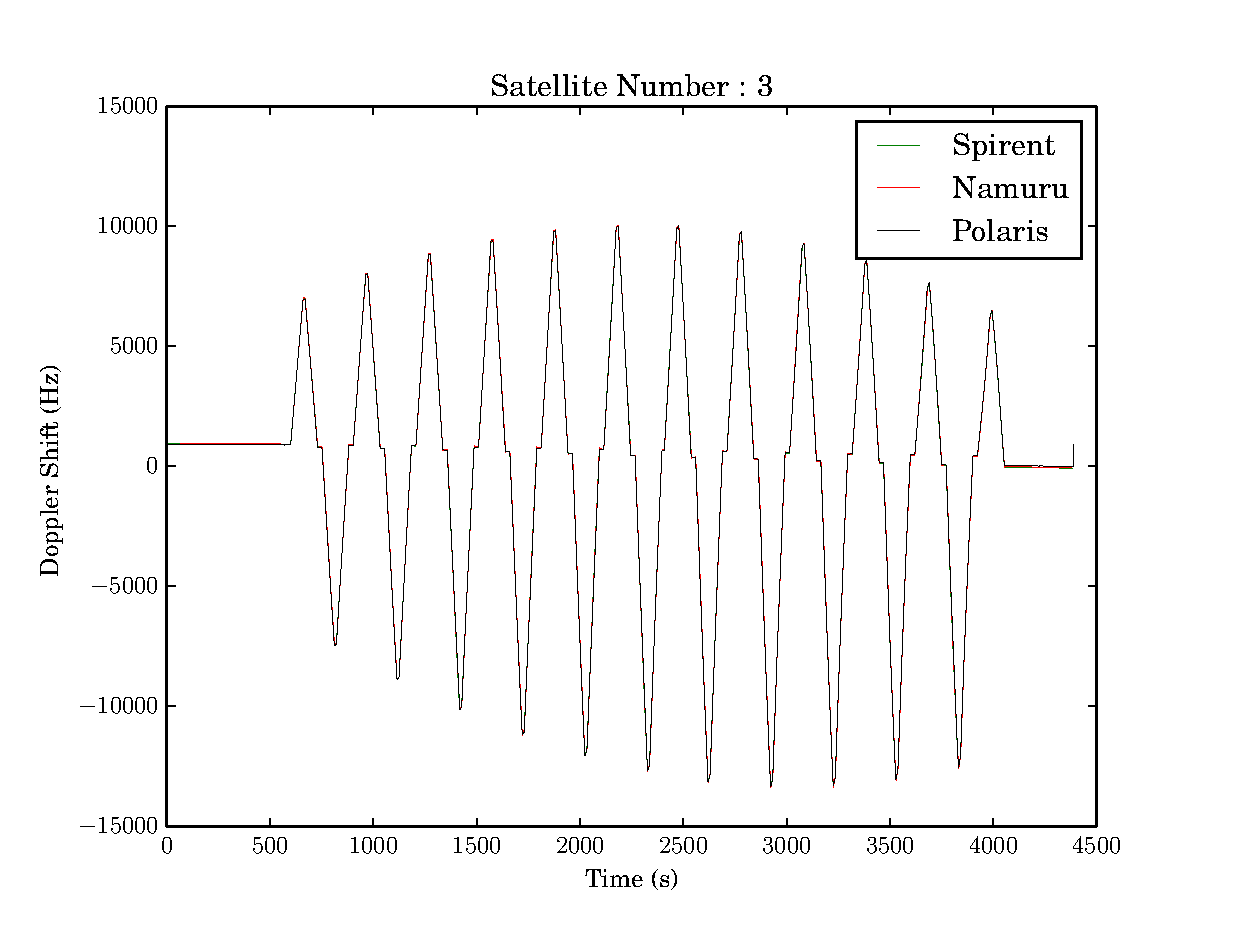
\includegraphics[width=1\textwidth]{PolarisCharts/3Polaris.eps} 
    \caption{An example of a simulation. This scenario, called  "HIGHG3" is designed to stress test the receiver by exposing it to high dynamics, in particular velocities of up to 9,000m/s and 15g. The scenario was generated using the \emph{SimGen} software which can be seen in figure \ref{fig:HighGScreenshot}.}
    \label{fig:Polaris3}
\end{figure}


\begin{figure}[!htb] 
    \centering
    \includegraphics[width=1\textwidth]{mywork/Spirent-GSS8000.jpg} 
    \caption{An example of a Spirent \ac{GPS} simulator. The actual model used for this research differs from the one pictured. The simulator is controlled by a tethered computer, which runs the \emph{SimGen} software, pictured in figure \ref{:HighGScreenshot}.}
    \label{fig:Spirent}
\end{figure}

\begin{figure}[!htb] 
    \centering
    \includegraphics[width=1\textwidth]{mywork/HighGScreenshot.png} 
    \caption{The SimGen software, used to define scenarios and control the \ac{GNSS} simulator.}
    \label{:HighGScreenshot}
\end{figure}


The correct performance of a \ac{PLL} can be examined by attempting to decode the navigation message transmitted by the satellite. Other, more sophisticated methods for determining if the  receiver is in phase lock, will be examined in Thesis B. In figures \ref{fig:RawSignal} and \ref{fig:DigitalSignal}, the decoded message can be clearly seen, indicating that the receiver is maintaining phase lock with the signal.

\subsection{Software simulation}
\ref{ch:Code}

\section{Airborne experiment}

\begin{figure}[!htb] 
    \centering
    \includegraphics[width=1\textwidth]{mywork/SeminoleBankingPRjpg.jpg} 
    \caption{A Piper PA-44 Seminole.}
    \label{fig:PiperSeminole}
\end{figure}

A real-world data-set was processed, consisting of data taken captured a flight aboard a UNSW Aviation Piper PA-44 Seminole VH-FRI. Data from the flight was captured by a NordNav IF Recorder, and processed using the the software receiver. 

The actual carrier doppler shift, as measured by taking the finite difference of the satellite pseudoranges, and converted to Hz, was compared against the measured Doppler shift in the software receiver. There is a small offset because of drift in the receiver crystal. The results of this experiment can be see in figure \ref{fig:SimulatedDynamics}. While the dynamics experienced by the receiver were on the order of $\pm 5m/s^2$, somewhat less than the dynamics that are experienced by a \ac{LV}, This experiment is important, as it verifies the real world performance of the soft receiver. 

\section{Modifications to receiver}

\subsection{New Coefficients}

